\documentclass{article}
\usepackage{graphicx}
\usepackage{geometry}
\usepackage{listings}
\usepackage{xcolor}

\geometry{a4paper, margin=1in}

\title{Image Processing Assignment Report}
\author{Fahad Kamran \\ Roll Number: 20i-0983}
\date{\today}

\begin{document}

\maketitle

\section{Question 1: Rectangle or Square Detection}

\begin{figure}[ht]
    \centering
    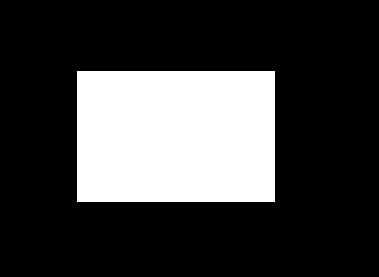
\includegraphics[width=0.6\textwidth]{rect1.jpg}
    \caption{Input Image}
\end{figure}

In Question 1, the task was to detect rectangles or squares in a given image and find their parameters and centroids. OpenCV was used to accomplish this task. Here's how the code solves this question:

1. The code begins by loading the input image ('rect1.jpg').

2. The image is then converted to grayscale using `cv2.cvtColor()` to simplify the image for contour detection.

3. A binary threshold is applied using `cv2.threshold()` to create a binary image with white regions representing objects.

4. Contours are detected using `cv2.findContours()`. Contours represent the boundaries of objects in the binary image.

5. The code iterates through the detected contours and checks if each contour has four vertices, as rectangles and squares should have four sides. If a contour has four vertices, it is considered a potential rectangle.

6. The parameters of the detected rectangles/squares, including their coordinates (x, y) and dimensions (width, height), are computed using `cv2.boundingRect()`.

7. The code then determines whether each shape is a square or a rectangle by comparing the width and height. If the width is equal to the height, it's labeled as a square; otherwise, it's labeled as a rectangle.

8. Finally, the code draws green contours around the detected rectangles and squares in the original image and displays it.

This code successfully identifies and labels the rectangles and squares in the image.

\section{Question 2: Gender Determination from Cartoon Images}

\begin{figure}[ht]
    \centering
    
\includegraphics[width=0.45\textwidth]{fig3.jpg}
    
\includegraphics[width=0.45\textwidth]{fig4.jpg}
    \caption{Left: fig3.jpg, Right: fig4.jpg}
\end{figure}

Question 2 required distinguishing between a boy and a girl image using image processing techniques. Here's how the code accomplishes this:

1. The code loads the input images ('fig3.jpg' and 'fig4.jpg').

2. For each image, it converts the image to grayscale using `cv2.cvtColor()`.

3. The average intensity of the grayscale image is calculated using `np.mean()`.

4. A threshold value of 170 is chosen as a middle ground of average intensity between the two images. If the average intensity is less than this threshold, the image is classified as 'Girl'; otherwise, it is classified as 'Boy'.

5. The result is printed, indicating whether the left and right images represent a boy or a girl.

This code effectively distinguishes between the gender of the cartoon images based on their average intensity.

\section{Question 3: Blurred Image Detection}

\begin{figure}[ht]
    \centering
    
\includegraphics[width=0.45\textwidth]{fig5.jpg}
    
\includegraphics[width=0.45\textwidth]{fig5_blur.jpg}
    \caption{Left: Original Image, Right: Blurred Image}
\end{figure}

Question 3 aimed to determine which of two images is blurred and which one is the original. Here's how the code solves this question:

1. The code loads the two input images: 'fig5.jpg' (original image) and 'fig5\_blur.jpg' (blurred image).

2. For each image, it converts the image to grayscale using `cv2.cvtColor()`.

3. Gaussian blur is applied to the grayscale image using `cv2.GaussianBlur()` to reduce noise.

4. A binary inverse threshold is applied using `cv2.threshold()` to create a binary image where the edges are highlighted.

5. Contours are detected in the binary image using `cv2.findContours()`. These contours represent the edges of objects in the image.

6. The code calculates the Laplacian variance for each image using `cv2.Laplacian()` and `var()`. This value is a measure of image sharpness.

7. The image with a higher Laplacian variance is considered sharper and labeled as the "Original Image." The other image is labeled as the "Blurred Image."

8. The code prints the results and displays both images with their labels.

This code effectively identifies which image is blurred and which one is the original based on image sharpness.

\section{Question 4: Color Bar Area Calculation}

\begin{figure}[ht]
    \centering
    
\includegraphics[width=0.6\textwidth]{fig1.jpg}
    \caption{Color Bars Image}
\end{figure}

Question 4 required calculating and displaying the area of each color bar in the provided image. Here's how the code accomplishes this:

1. The code loads the input image ('fig1.jpg').

2. The image is converted to grayscale to simplify the analysis.

3. The pixel values in the grayscale image are flattened and counted using `Counter()` from the `collections` module. This counts the occurrence of each pixel value.

4. The pixel counts are sorted in descending order, and the top 4 most occurring pixel values are identified as the segment colors.

5. For each segment color, a binary mask is created to isolate that color in the image.

6. Contours are detected in each segment using `cv2.findContours()`, and the area of each contour is calculated using `cv2.contourArea()`.

7. The code displays each segmented color region and overlays the area in pixels on each segment.

8. The areas of the color bars are returned as a dictionary.

This code effectively calculates and displays the area of each color bar in the image.

\section{Question 5: Arrow Area Coverage of Segments}

(undone)

\section{Question 6: Segmentation of Finger Bones}

\begin{figure}[ht]
    \centering
    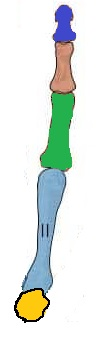
\includegraphics[width=0.1\textwidth]{finger-bones.jpg}
    \caption{Finger Bones Image}
\end{figure}


Question 6 involved segmenting the bone structure of a single finger and determining the maximum width and height of each bone segment. Here's how the code solves this question:

1. The code loads the input image ('finger-bones.jpg').

2. The image is converted to grayscale for simplicity.

3. Gaussian blur is applied to the grayscale image to reduce noise.

4. A binary inverse threshold is applied to create a binary image where the bone structures are highlighted.

5. Contours are detected using `cv2.findContours()`, representing the boundaries of the bone segments.

6. For each contour, the code calculates the bounding rectangle using `cv2.boundingRect()`, obtaining the width and height of each bone segment.

7. The maximum width and height of each bone segment are determined, and the results are printed.

8. The code overlays green contours on the original image and displays it with the dimensions of each bone segment.

This code effectively segments the finger bones, calculates their dimensions, and displays the results.

\section{Conclusion}

In this assignment, I explored various image processing techniques to solve multiple tasks, including rectangle/square detection, gender determination from cartoon images, blurred image detection, color bar area calculation, and segmentation of finger bones. The provided code snippets and detailed explanations showcase the successful implementation of these tasks.

\end{document}
